Una masa m está unida arriba a un soporte fijo mediante un resorte \(k_1\) y un amortiguador \(c_2\) en paralelo. Un segundo resorte \(k_3\) une la masa al apoyo inferior móvil P. Los desplazamientos x de la masa y f de P se miden hacia abajo desde el equilibrio inicial. Inicialmente \(x(0)\)=\(x'(0)\)=0. Los parámetros, en SI, son \(k_1=2\,\mathrm{N/m}\), \(c_2=5\,\mathrm{N\,s/m}\), \(k_3=3\,\mathrm{N/m}\), \(m=1\,\mathrm{kg}\). Se consideran resortes y amortiguador lineales.

\begin{enumerate}[label=(\alph*),ref=\alph*,leftmargin=*]
\item Halla x(t) si \(f(t)=\sin(2t)\,\mathrm{cm}\).
\item Halla x(t) si P baja a velocidad 0.01 m/s durante 10 s y luego permanece inmóvil.
\item Clasifica el amortiguamiento y calcula su razón \(\zeta\).
\end{enumerate}

\Needspace{9.030000000000001cm}
\begin{center}
\begin{minipage}{\linewidth}
\centering
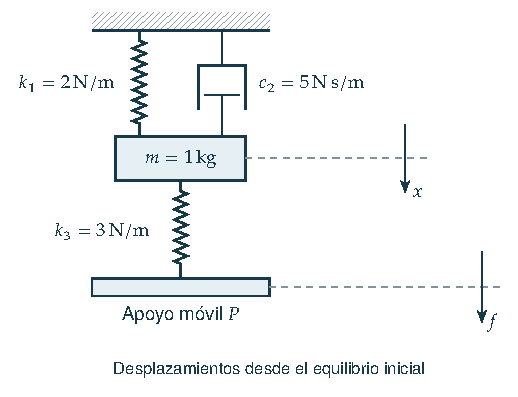
\includegraphics[width=9.83cm]{assets/M2-E0129-setup.pdf}\par
\smallskip{\small Conexiones de la masa con el soporte fijo y el apoyo móvil.\par}
\end{minipage}
\end{center}
